% !TeX spellcheck = en_US
% !TeX encoding = UTF-8
\documentclass[11pt, a4paper, final]{amsart}
\setlength{\emergencystretch}{2em}


\usepackage[T1]{fontenc}
\usepackage{lmodern}
\usepackage{mathtools}
%\usepackage[activate={true,nocompatibility},final,tracking=true,kerning=true,spacing=true,stretch=10,shrink=10]{microtype}
%\microtypecontext{spacing=nonfrench}
\usepackage[utf8]{inputenc}

\topmargin0pt
\oddsidemargin0pt
\evensidemargin0pt
\textheight660pt
\textwidth445pt

\usepackage{amsfonts}
\usepackage{amsmath}
\usepackage{amssymb}
\usepackage{amsthm}
\usepackage{mathtools}
\usepackage{paralist, tabularx}
\usepackage{enumerate}
\usepackage[utf8]{inputenc}
\usepackage{mathabx,epsfig}
\usepackage{tikz-cd}

\usepackage{verbatim}

\usepackage{etoolbox}


%tikz pacakges and settings 
\usepackage{tikz}
\usetikzlibrary{decorations.markings, calc, tqft}
\usetikzlibrary{decorations.pathmorphing}
\tikzset{mid arrow/.style={
    postaction={decorate},
    decoration={markings, mark=at position 0.5 with {\arrow{stealth}}}
}}


\usepackage{xcolor}
\definecolor{green}{RGB}{0,127,0}
\definecolor{redd}{RGB}{191,0,0}
\definecolor{red}{RGB}{105,89,205}
\usepackage[colorlinks=true]{hyperref}

\usepackage[notref, notcite]{showkeys}
\usepackage[cmtip,arrow]{xy}

%%%%%%%%%%%%%%%%%%%%%%%%%%%%%%%%%%%%%%%%%%%%%%%%%%%%%%%%%%%%%%%%
\begin{comment}
\usepackage[backend=biber,
url=false,
isbn=false,
backref=true,
citestyle=alphabetic,
bibstyle=alphabetic,
autocite=inline,
maxnames=99,
minalphanames=4,
maxalphanames=4,
sorting=nyt,]{biblatex}
\addbibresource{two_three_steps.bib}
\end{comment}

\usepackage{filecontents}
\begin{filecontents}{references.bib}

\end{filecontents}

\usepackage[
backend=bibtex,
%style=alphabetic,
url=false,
isbn=false,
backref=true,
citestyle=alphabetic,
bibstyle=alphabetic,
autocite=inline,
maxnames=99,
minalphanames=4,
maxalphanames=4,
sorting=nyt,
]{biblatex}

\addbibresource{references.bib}
%%%%%%%%%%%%%%%%%%%%%%%%%%%%%%%%%%%%%%%%%%%%%%%%%%%%%%%%%%%%%%%%


\DeclareMathOperator{\Aut}{Aut}
\DeclareMathOperator{\Sym}{Sym}
\DeclareMathOperator{\Hom}{Hom}
\newcommand{\R}{{\mathbb{R}}}
\newcommand{\Z}{{\mathbb{Z}}}
\newcommand{\N}{{\mathbb{N}}}
\newcommand{\LL}{\mathcal{L}}
\newcommand{\FF}[1]{\mathbb{F}_{#1}}
\DeclareMathOperator{\error}{{error}}
\DeclareMathOperator{\Mor}{Mor}
\DeclareMathOperator{\id}{id}

\newcommand{\C}{\mathfrak{C}}
\newcommand{\M}{{\mathcal M}}


\newcommand\todo[1]{\textbf{\textcolor{redd}{#1}}}


\newcommand{\nref}[2]{\hyperref[#1]{\ref*{#1}$_{#2}$}}

\newcommand{\cupdot}{\mathbin{\mathaccent\cdot\cup}}


\DeclareMathOperator{\topo}{{top}}
\DeclareMathOperator{\im}{{Im}}
\DeclareMathOperator{\lin}{{Lin}}
\DeclareMathOperator{\Th}{{Th}}
\DeclareMathOperator{\SL}{{SL}}
\DeclareMathOperator{\tp}{{tp}}
\DeclareMathOperator{\cl}{{cl}}
\DeclareMathOperator{\dcl}{{dcl}}

%%%%%%%%%%%%%%%%%%%%%%%%%%%%%%%%%%%%%%%%%%%%%%%%%%%%%%%%%%%% NASZE KOMENDY %%%%%%%%%%%%%%%%%%%%%%%%%%

\newcommand{\unit}{\mathcal{I}}
\newcommand{\sphere}{\mathcal{S}}
\newcommand{\disk}{\mathcal{D}}
\newcommand{\pt}{\star}

\DeclareMathOperator{\const}{{const}}

\DeclareMathOperator{\SO}{SO}
\DeclareMathOperator{\Ext}{Ext}
\DeclareMathOperator{\Tor}{Tor}

%%%%%%%%%%%%%%%%%%%%%%%%%%%%%%%%%%%%%%%%%%%%%%%%%%%%%%%%%%%%%%%%%%%%%%%%%%%%%%%%%%%%%%%%%%%%%%%%%%%%%


\newtheorem{theorem}{Theorem}
\numberwithin{theorem}{section}
\newtheorem{lemma}[theorem]{Lemma}
\newtheorem{claim}[theorem]{Claim}
\newtheorem{fact}[theorem]{Fact}
\newtheorem{proposition}[theorem]{Proposition}
\newtheorem{problem}[theorem]{Problem}
\newtheorem{conjecture}[theorem]{Conjecture}
\newtheorem{axiom}[theorem]{Axiom}
\newtheorem{question}[theorem]{Question}
\newtheorem{corollary}[theorem]{Corollary}
\newtheorem*{theorem2}{Theorem}
\newtheorem*{claim2}{Claim}
\newtheorem*{corollary2}{Corollary}
\newtheorem*{question2}{Question}
\newtheorem*{conjecture2}{Conjecture}


\newtheorem{clm}{Claim}
\newtheorem*{clm*}{Claim}


\theoremstyle{definition}
\newtheorem{definition}[theorem]{Definition}
\newtheorem*{definition2}{Definition}
\newtheorem{example}[theorem]{Example}

\theoremstyle{remark}
\newtheorem{remark}[theorem]{Remark}
\newtheorem*{remark2}{Remark}


\AtEndEnvironment{proof}{\setcounter{clm}{0}}
\newenvironment{clmproof}[1][\proofname]{\proof[#1]\renewcommand{\qedsymbol}{$\square$(claim)}}{\endproof}

\usepackage[hyphenbreaks]{breakurl}

%\usepackage{filecontents}
%\begin{filecontents}{references.bib}

%\end{filecontents}

\usepackage[
backend=bibtex,
%style=alphabetic,
url=false,
isbn=false,
backref=true,
citestyle=alphabetic,
bibstyle=alphabetic,
autocite=inline,
maxnames=99,
minalphanames=4,
maxalphanames=4,
sorting=nyt,
]{biblatex}

\usepackage{calligra}


%\addbibresource{references.bib}

\title{Hatcher solutions}

\author{Michał Mądrala}
\author{Ruba Rudzik}
\author{Krzysztof Szymański}

\begin{document}

	\begin{abstract}
	       We present the solutions to the excercises found in Allen Hatcher's ,,Algebraic Topology'' \cite{AH} with our own perspective and commentary. We also present proofs of selected theorems (with what we hope is a more detailed explanation). 
	\end{abstract}
	
\maketitle

\begin{center}
    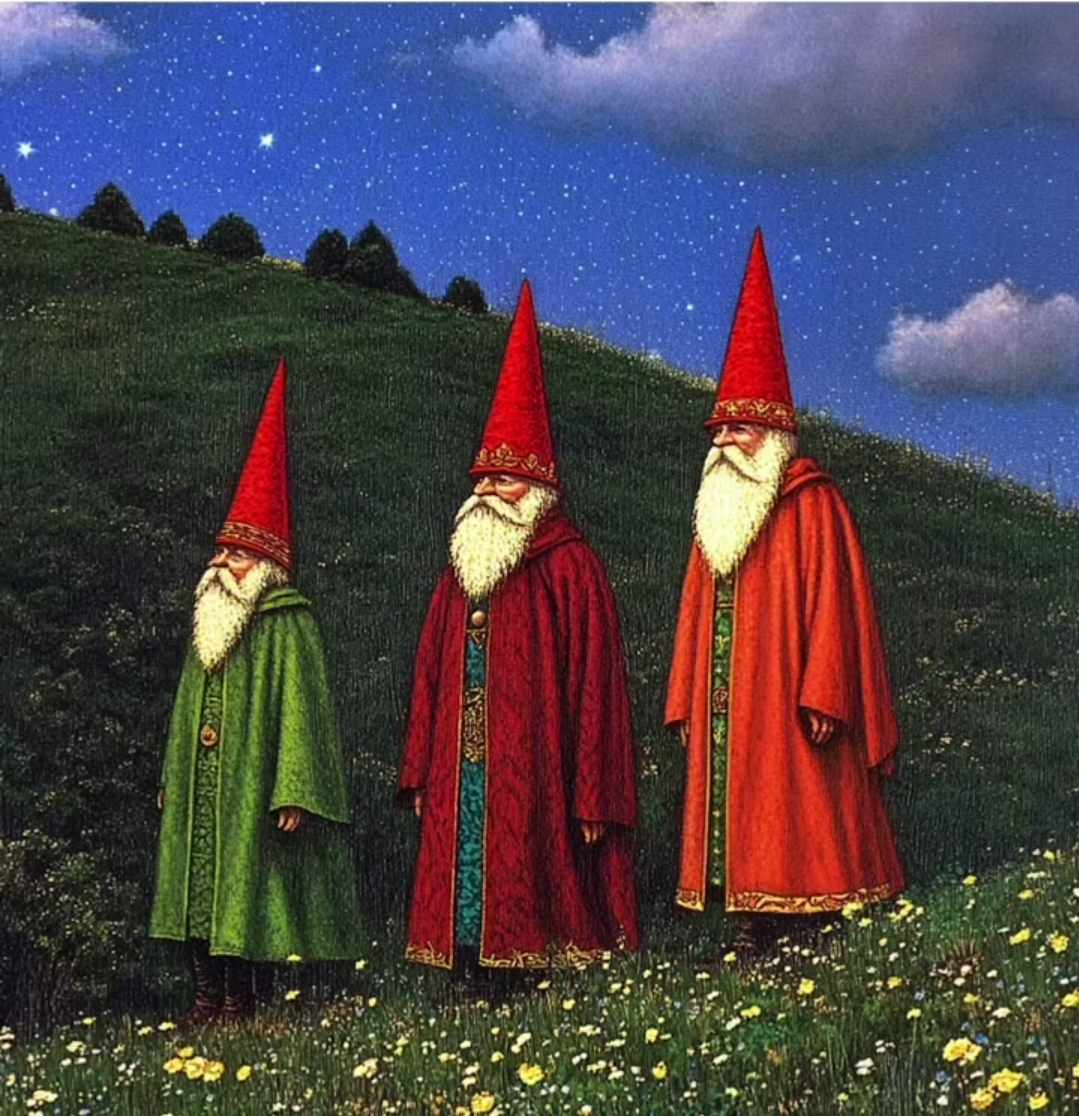
\includegraphics[width=120mm]{images/jd_śwg_jśw.jpg}
\end{center}

\begin{center}
    {\fontfamily{pzc}\selectfont Dedicated to Jan Dymara, Światosław Gal \& Jacek Świątkowski}
    %{\calligra Dedicated to Jan Dymara, Swiatoslaw Gal, Jacek Świątkowski}
\end{center} 

\newpage

\section{Introduction}

\todo{Blabla że co w ogóle robimy...}

We denote a $k$-sphere by $\sphere^k$, $k$-disk by $\disk^k$ and a $[0, 1]$ segment by $\unit$. By $\simeq$ we mean homotopy or, when placed between spaces, homotopy equivalence when placed between spaces. We denote homeomorphisms by $\approx$.


\section{The Fundamental Group}

\subsection{Basic Constructions}

This section is about basic constructions.

\todo{Należałoby poprawić numerację problemów, żeby była tak jak w hatcherze, no i też żeby sekcje w Additional Topics nie były 2.4 itp tylko 2.A, 2.B itd}

\begin{problem}[1.1.1]\label{problem: 1.1.1}
Show that composition of paths satisfies the following cancellation property: If
$f_0 \cdot g_0 \simeq f_1 \cdot g_1$ and $g_0 \simeq g_1$ then $f_0 \simeq f_1$.
\end{problem}

\begin{proof}
    The homotopy assumptions imply that $g_i$ have the same endpoints, and so do the $f_ig_i$, which means the $f_i$ have the same endpoints as well.

    Since $g_0 \simeq g_1$, it is clear that $\bar{g_0} \simeq \bar{g_1}$. We proceed as shown on the homotpy diagram:

    \begin{center}
        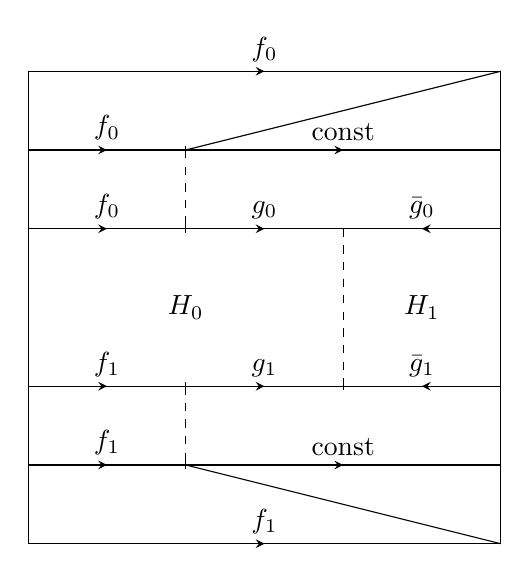
\begin{tikzpicture}

%0
\draw (0,0) rectangle (6,6);
\draw[mid arrow] (0,0) -- node[anchor = south]{$f_1$} (6,0);

%1
\draw (2,1) -- (6,0);
\draw[mid arrow] (0,1) -- node[anchor = south]{$f_1$} (2,1);
    \draw (2,0.95) -- (2,1.05);
\draw[mid arrow] (2,1) -- node[anchor = south]{const} (6,1);

%2
\draw[mid arrow] (0,2) -- node[anchor = south]{$f_1$} (2,2);
    \draw (2,1.95) -- (2,2.05);
    \draw[dashed] (2,2) -- (2,1);
\draw[mid arrow] (2,2) -- node[anchor = south]{$g_1$} (4,2);
    \draw (4,1.95) -- (4,2.05);
\draw[mid arrow] (6,2) -- node[anchor = south]{$\bar{g}_1$} (4,2);

%4
\draw[mid arrow] (0,4) -- node[anchor = south]{$f_0$} (2,4);
    \draw (2,3.95) -- (2,4.05);
\draw[mid arrow] (2,4) -- node[anchor = south]{$g_0$} (4,4);
    \draw[dashed] (4,4) -- (4,2);
    \node at (2,3) {$H_0$};
\draw[mid arrow] (6,4) -- node[anchor = south]{$\bar{g}_0$} (4,4);
    \node at (5,3) {$H_1$};

%5
\draw[mid arrow] (0,5) -- node[anchor = south]{$f_0$} (2,5);
    \draw (2,4.95) -- (2,5.05);
    \draw[dashed] (2,5) -- (2,4);
\draw[mid arrow] (2,5) -- node[anchor = south]{const} (6,5);
    \draw (2,5) -- (6,6);

%6
\draw[mid arrow] (0,6) -- node[anchor = south]{$f_0$} (6,6);

\end{tikzpicture}
    \end{center}
    Algebraically, this corresponds to the computations
    % TODO: operator for const to improve the spacing
    \[
    f_0 \simeq f_0 \,\mathrm{const}_{x_0} \simeq f_0(g_0\overline{g_0}) \simeq (f_0g_0)\overline{g_0} \simeq (f_1g_1)\overline{g_1} \simeq f_1(g_1\overline{g_1})  \simeq f_1\,\mathrm{ const}_{x_0} \simeq f_1,
    \]
    where \(x_0\) denotes the enpoint of the paths $f_i$.
\end{proof}

\begin{problem}[1.1.2]\label{problem: 1.1.2}
    Show that the change-of-basepoint homomorphism $\beta_h$ depends only on the homotopy class of $h$.
\end{problem}

\begin{proof}
    It suffices to show that for every two homotopic loops $h$ and $h'$ we have $\beta_h = \beta_{h'}$. Let $H$ denote the homotopy $h \simeq_{H} h'$. Take any loop $g$. We have that $\beta_h(g) = hg\overline{h} \simeq h'g\overline{h'} = \beta_{h'}(g)$. \todo{obrazek}
\end{proof}

\begin{problem}[1.1.3]\label{problem: 1.1.3}
    For a path-connected space \(X\), show that \(\pi_1(X)\) is abelian iff all basepoint-change homomorphism \(\beta_h\) depend only on the endpoints of the path \(h\).
\end{problem}

\begin{proof}
    ($\Rightarrow$)
    Consider any two paths $h,h'$ from points $y \in X$ to $x \in X$. We want to show that $\beta_h = \beta_{h'}$. Consider any loop $g \in \pi_1(X,x)$ and a loop $\bar{h}h'$ which also is in $\pi_1(X,x)$. Since $\pi_1(X)$ is abelian then $\pi_1(X,x)$ is also abelian. And so it follows that:
    \[
        g\cdot \bar{h}h' \simeq \bar{h}h' \cdot g 
    \]
    Now multiply it by $h$ on left hand side, and by $\bar{h'}$ on right hand side to get: 
    \[
        hg\bar{h} \simeq h'g\bar{h'}
    \]
    That is exactly equivalent to $\beta_h =\beta_{h'}$. \\

    ($\Leftarrow$) Suppose that for any two paths from $x$ to $y$ they induce the same maps $\beta_h,\beta_{h'}$. In particular given any two loops $g,h$ in $\pi_1(X,x_0)$ we have $\beta_g = \beta_h$. And so it follows that:
    \[
    hg\bar{h}= \beta_h(g) =\beta_g(g)=g
    \]
    Thus $gh = hg$ which means that $\pi_1(X,x)$ is abelian, and so of course $\pi_1(X)$ is abelian too.
\end{proof}

\begin{problem}[1.1.4]\label{problem: 1.1.4.}
    A subspace \(X \subseteq \mathbb{R}^n\) is said to be \emph{star-shaped} if there is a point \(x_0 \in X\) such that for each \(x \in X\) the line segment from \(x_0\) to \(x\) lies in \(X\). Show that if a subspace \( X \subseteq \mathbb{R}^n\) is locally star-shaped, in the sense that every point of \(X\) has a star-shaped neighbourhood in \(X\), then every path in \(X\) is a piecewise linear path, that is, a path consisting of a finite number of straight lines traversed at constant speed. Show that this applies in particular when \(X\) is open or when \(X\) is a union of finitely many closed convex subsets.
\end{problem}

\begin{proof}
In the case that \(X\) is star-shaped as a whole, it is contractible, so the thesis definitely holds. Denote the path in question by \(\gamma\). In general, we can use the compactness of the image of \( \gamma \) to cover it with finitely many star-shaped sets. However, in each of these we cannot just contract the curve, as we must keep the endpoints intact. 

Instead we show the following: if \(X\) is star-shaped with \emph{star-point} \(x_0\), we can deform any path \(\gamma\) in \(X\) to a linear path going from \(\gamma(0)\) to \(x_0\) and then from \(x_0\) to \( \gamma(1) \). Without loss of generality \(x_0 = 0\). The homotopy given by
\todo{Obrazek} 
\[
H_1(s,t) = \Bigl [ (1-t) + t|1 - 2s| \Bigr ] \gamma(s)
\]
achieves this partially, as it deforms \(\gamma(s)\) to \(|1 - 2s|\gamma(s)\), which is equal to \(\gamma(0), x_0, \gamma(1)\) at \(s=0, \frac{1}{2}, 1\). Now we turn to making the segments linear.

If \( \delta \) is the first half of \(\gamma\), the homotopy \(H_1\) deforms it to the path \((1-s)\delta(s)\). We will deform it to \(s\delta(0)\), which is certainly constant-speed. This is achieved through the homotopy
\[
H_2(s,t) = (1-s)\delta\bigl((1-t)s\bigr).
\]
Finally, applying the same procedure to the second half of \(\gamma\), we will have indeed deformed \(\gamma\) to a piecewise-linear path consisting of two segments. 
\end{proof}

\begin{proof}[Open sets.]
    In an open set, every point has a neighbourhood which is a Euclidean ball, so the space \(X\) is locally star-shaped.
\end{proof}

\begin{proof}[Finite unions of convex sets.] Call a subspace \(X \subseteq \mathbb{R}^n\) \emph{strictly locally star-shaped} iff every \(x \in X\) has a star-shaped neighbourhood \emph{for which it is the star-point}. Every convex set satisfies this property. We will show that if \(A\) and \(B\) are closed and strictly locally star-shaped, then so is their union.

Pick a point \( x \in A \cup B \). Without loss of generality, \( x \in A\). Then either \( x \in B\) or \( x \) is separated from \(B\). In the first case, for some small \( r \) we have a neighbourhood
\[
B_r(x) \cap X = (B_r(x) \cap A) \cup (B_r(x) \cap B),
\]
which is the union of star-shaped neighbourhood with the same star-point, so it is star shaped. In the second case, for some small \(r\) we have
\[
B_r(x) \cap X = B_r(x) \cap A,
\]
so \(x\) has a star-shaped neighbourhood.
\end{proof}

\begin{problem}[1.1.5]\label{problem: 1.1.5.}
    Show that for a space \(X\), the following three conditions are equivalent:
    \begin{enumerate}[(a)]
        \item Every map \( \sphere^1 \longrightarrow X\) is homotopic to a constant map, with image a point.
        \item Every map \(\sphere^1 \longrightarrow X\) extends to a map \(\disk^2 \longrightarrow X\).
        \item \( \pi_1(X, x_0) = 0 \) for all \( x_0 \in X\).
    \end{enumerate}
    Deduce that a space \(X\) is simply-connected all maps \(\sphere^1 \longrightarrow X\) are homotopic. [In this problem, 'homotopic' means 'homotopic without regard to basepoints'.]
\end{problem}

\begin{proof} 
    ($a \Rightarrow b$) Take any $f : \sphere^1 \rightarrow X$. We have that $f \simeq_H \const_{x_0}$ for some $x_0 \in X$, with a homotopy $H: \sphere^1 \times \unit \rightarrow X$. Since $H(x, 0) = f(x)$ and $H(x, 1) = x_0$ we can consider the quotient of $\sphere^1 \times \unit$ by the relation identifying $\sphere^1 \times \{1\}$ with a single point. Such a cone-like space is clearly homeomorphic with $\disk^2$. Let $j : \sphere^1 \times \unit \rightarrow \disk^2$ be the quotient map. We have the induced map $H'$ as shown in the diagram:
    
    \[\begin{tikzcd}
	{\sphere^1} & {\sphere^1 \times \unit} & {\disk^2} \\
	& X
	\arrow["i", hook, from=1-1, to=1-2]
	\arrow["f"', from=1-1, to=2-2]
	\arrow["j", two heads, from=1-2, to=1-3]
	\arrow["H"', from=1-2, to=2-2]
	\arrow["{H'}", from=1-3, to=2-2]
    \end{tikzcd}\]

    Now observe that $H' \circ j \circ i$ extends $f$ to a disk. \\

    ($b \Rightarrow c$) \todo{obrazek} Take any $g \in \pi_1(X,x_0)$. It can be represented as a map $g : \sphere^1 \to X$ and by assumption we get $\bar{g} : \disk^2 \to X$ which extends $g$. Suppose that $s \in \disk^2$ corresponds to the base point $x_0$ by $g$. Since disks are contractible we get homotopy $H$ that in $0$ is the boundary sphere $\sphere^1$ and in $1$ it is a point in the middle of $D^2$ and call it $m$. Now consider a path $h$ from point $s$ to $m$ as in the diagram. The homotopy $H$ contracts path $h$ to a constant path in $m$. We will now show that $\beta_h(g) = 0 \in \pi_1(X,\bar{g}(m))$. Since $\beta_h(g) = hg\bar{h}$ we conclude that $H$ contracts $hg\bar{h}$ to a point $\bar{g}(m)$, which is exactly representation of $0$ in $\pi_1(X,\bar{g}(m))$. Because $\beta_h$ is isomorphism we see that $g$ must be in the same class as trivial map in $\pi_1(X,x_0)$. \\

    ($c \Rightarrow a$)

    Since $\pi_1(X,x_0)$ is trivial, every loop is homotopic to a constant loop. Lets call this homotopy $H$. Since every loop can be represented as a map $\sphere^1 \to X$, by simply taking the homotopy $H$ we get the thesis.
\end{proof}

\begin{problem}[1.1.6]\label{problem: 1.1.6}
    We can regard $\pi_1(X, x_0)$ as the set of basepoint-preserving homotopy classes of maps $(\sphere^1, s_0) \rightarrow (X, x_0)$. Let $[\sphere^1, X]$ be the set of homotopy classes of maps $\sphere^1 \rightarrow X$ with no conditions on basepoints. Thus there is a natural map $\Phi : \pi_1(X, x_0) \rightarrow [\sphere^1, X]$ obtained by ignoring basepoints. Show that $\Phi$ is onto if $X$ is path-connected, and that $\Phi([f]) = \Phi([g])$ iff $[f]$ and $[g]$ are conjugate in $\pi_1(X, x_0)$. Hence $\Phi$ induces a one-to-one correspondence between $[\sphere^1, X]$ and the set of conjugacy classes in $\pi_1(X)$ when $X$ is path-connected.
\end{problem}

\begin{problem}[1.1.7]\label{problem: 1.1.7}
    Define $f:\sphere^1 \times \unit \to \sphere^1 \times \unit$ by $f(\theta, s) = (\theta + 2\pi s , s)$, so $f$
    restricts to the indentity  on the two boundary circles of $\sphere^1 \times \unit$. Show that $f$ is homotopic to 
    the identity by a homotopy $f_t$ that is stationary on one of the boundary circles, but not by any homotopy $f_t$
    that is stationary on both boundary cricles.   
\end{problem}

\begin{proof}
    For the first part definie homotpy $f_t : \sphere^1 \times \unit \times \unit \to \sphere ^2 \times \unit$ as follows:

    \begin{equation}
        f_t(\theta, s) = (\theta  + 2 \pi s (1 - t) , s)
    \end{equation}

    This ofcource is stationary on $\sphere \times \{0\}$ because the term $2 \pi s (1 - t)$ vanishes for $s = 0$ for all $t$, but
    we see that is not stationary on the boundary circle $\sphere^1 \times \{1\}$

    For the second part consider a loop $\gamma(t) = (\theta_0,t)$, where $\theta_0$ is a point on $\sphere^1$. The image of $\gamma$ under
    map $f$ will be a path connecting points $(\theta_0, 0)$ and $(\theta_0, 1)$ and going around the cylinder once (As pictured below).
    \begin{center}
        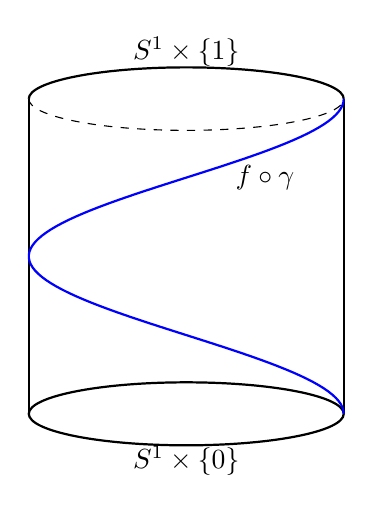
\begin{tikzpicture}[scale=2]

  \draw[thick] (0,0) ellipse (1 and 0.2);

  \draw[thick] (-1,0) -- (-1,2);
  \draw[thick] (1,0) -- (1,2);

  \draw[dashed] (-1, 2) arc (180:360:1 and 0.2);
  \draw[thick]  (1, 2) arc (0:180:1 and 0.2);

  \draw[blue, thick, domain=0:360, samples=100, variable=\t]
    plot ({cos(\t)}, {2*\t/360});

  \node at (0,-0.3) {$S^1 \times \{0\}$};
  \node at (0,2.3) {$S^1 \times \{1\}$};
  \node at (0.5,1.5) {$f \circ \gamma$};

\end{tikzpicture}
    \end{center}

    Now suppose for contradiction that there is homotopy $f_t$ that is stationary on both boundary. Then we would be able to
    construct homotopy between paths $f \circ \gamma$ and $\gamma$. Now consider loop based in $\theta_0$ $(f \circ \gamma) \cdot \bar{\gamma}$
    This loops is nontrivial generator of group $\pi(\sphere^1 \times \unit, \theta_0)$. But we get that:
    \begin{equation}
        (f \circ \gamma) \cdot \bar{\gamma} \simeq \gamma \cdot \bar{\gamma} \simeq \text{const}_{\theta_0}
    \end{equation}

    That is contradiction.
\end{proof}

\begin{problem}[1.1.8]\label{problem: 1.1.8}
    Does the Borsuk-Ulam theorem hold for the torus? In other words, for every map
    $f: \sphere^1 \times \sphere^1 \to \R^2$ must there exist $(x,y) \in \sphere^1 \times \sphere^1$ such that 
    $f(x,y)= f(-x,-y)$?
\end{problem}

\begin{proof}
    Consider torus embeded in $\R^3$ in the usual way and projection $\pi$ on to plane $z = 0$. 
    Ofcource if $\pi(a,b) = \pi(c,d)$ it must be that points $b = d$.
    So that automaticly contradicts the thesis of Borsuk Ulam theorem on Torus. 
\end{proof}

\begin{problem}[1.1.9]\label{problem: 1.1.9}
    Let $A_1 , A_2 , A_3$ be compact sets in $\R^3$ . Use the \textbf{Borsuk–Ulam theorem} to show
that there is one plane $P \subseteq \R^3$ that simultaneously divides each $A_i$ into two pieces of
equal measure.
\end{problem}

Let us introduce some notation. Let $\lambda$ denote the measure we are interested in. We can think of the set of all planes in $\R^3$, as $\sphere^2\times\R$, thus for a plane $P$, let $P_{n, t}$ denote the plane with a normal vector $n \in \mathcal{S}^2$, moved along it by $t \in \R$. We denote by $P^+_{n, t}, P^-_{n, t}$ two halves of $\R^3$, respectively above and below the $P_{n, t}$ (in the sense of direction of $n$). We will need the following lemma:

\begin{lemma}\label{lemma: about continous equal-cutting}
    Let $A \subseteq \R^3$ be a compact subset, there exists a continous, \textbf{even} map $h : \sphere^2 \xrightarrow{} \R$, such that:
    $$\lambda(P^+_{n, h(n)} \cap A) = \lambda(P^-_{n, h(n)} \cap A)$$
\end{lemma}

The idea behind the lemma is to find a continous family of planes, each equally dividing given set.
\todo{Zauważyliśmy, że potrzeba żeby ta mapa była parzysta.}

\begin{proof}\textit{(of the Lemma \ref{lemma: about continous equal-cutting})}
    \todo{TODO}
\end{proof}

\begin{proof}\todo{utworzyć begin-solution i tutaj zmienić)}
    Construct $h : \sphere^2 \to \R$ as in Lemma \ref{lemma: about continous equal-cutting} for $A_1$.
    Let $g : \sphere^2 \to \R^2$ be defined as follows:
    \[\begin{tikzcd}
	{\sphere^2} && {\R^2} \\
	n && {\begin{pmatrix}
	    \lambda(P^+_{n, h(n)} \cap A_2) \\
        \lambda(P^+_{n, h(n)} \cap A_3)
	\end{pmatrix}}
	\arrow["g", from=1-1, to=1-3]
	\arrow["\in"{marking, allow upside down}, draw=none, from=2-1, to=1-1]
	\arrow[maps to, from=2-1, to=2-3]
	\arrow["\in"{marking, allow upside down}, draw=none, from=2-3, to=1-3]
\end{tikzcd}\]
\todo{Ten diagram to tylko fleks z użycia quivera, można to napisać normalnie i pewnie będzie ładniej.} \\
Since $h$ is continous, $g$ is continous as well. By the \textbf{Borsuk-Ulam theorem}, there exists some $n \in \sphere^2$, such that:
$$\begin{pmatrix}
	    \lambda(P^+_{n, h(n)} \cap A_2) \\
        \lambda(P^+_{n, h(n)} \cap A_3)
	\end{pmatrix} = \begin{pmatrix}
	    \lambda(P^+_{-n, h(-n)} \cap A_2) \\
        \lambda(P^+_{-n, h(-n)} \cap A_3)
	\end{pmatrix} = \begin{pmatrix}
	    \lambda(P^-_{n, h(n)} \cap A_2) \\
        \lambda(P^-_{n, h(n)} \cap A_3)
	\end{pmatrix}$$
    The last equality follows from evenness of $h$, and the fact that $P^+_{-n, t} = P^-_{n, t}$.
    \todo{Zamiast tych pmatrixów można pisać $A_i$}
\end{proof}

\begin{problem}[1.1.10]\label{problem: 1.1.10}
    
\end{problem}

\begin{proof}
    Consider two loops $\alpha  \in X \times \{y_0\}$ and $\beta \in \{x_0\} \times Y$. They represents
    classes $[(\alpha, \text{const}_{y_0})]$ and $[(\text{const}_{x_0}, \beta)]$ (We use a little abuse of notation here) 
    The goal is to proof that 
    $$[(\alpha, \text{const}_{y_0})] [(\text{const}_{x_0}, \beta)] = [(\text{const}_{x_0}, \beta)][(\alpha, \text{const}_{y_0})] $$
    
    The diagram below show easy homotpy of loops: $\alpha \cdot \text{const}_{x_0} \simeq \text{const}_{x_0} \cdot \alpha$
    \begin{center}
        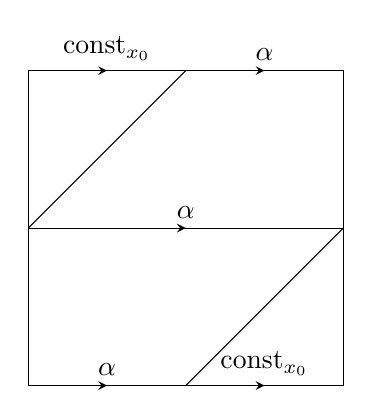
\begin{tikzpicture}

%0
\draw (0,0) rectangle (4,4);
\draw[mid arrow] (0,0) -- node[anchor = south]{$\alpha$} (2,0);
\draw[mid arrow] (2,0) -- node[anchor = south]{$\text{const}_{x_0}$} (4,0);
\draw (2,0) -- (4,2);

%1
\draw[mid arrow] (0,2) -- node[anchor = south]{$\alpha$} (4,2);
\draw (0,2) -- (2,4);

%2
\draw[mid arrow] (0,4) -- node[anchor = south]{$\text{const}_{x_0}$} (2,4);
\draw[mid arrow] (2,4) -- node[anchor = south]{$\alpha$} (4,4);

\end{tikzpicture}
    \end{center}

    We use this homotpy to construct the needed one to show the thesis. 

    \todo{Nie wiem czy tego nie dokładniej napisać jakoś?}
\end{proof}


\begin{problem}[1.1.14]\label{problem: 1.1.14}
    Show that the isomorphism $\pi_1(X \times Y) \cong \pi_1(X) \times \pi_1(Y)$ in \cite[Proposition 1.12]{AH} is given by $[f] \mapsto ({p_1}_*([f]), {p_2}_*([f]))$ where $p_1$ and $p_2$ are the projections of $X \times Y$ onto its two factors.
\end{problem}

\begin{problem}[1.1.15]\label{problem: 1.1.15}
    Given a map $f:X \rightarrow Y$ and a path $h : \unit \rightarrow X$ from $x_0$ to $x_1$, show that $f_*\beta_h = \beta_{fh}f_*$, namely that the diagram below commutes.

    \[\begin{tikzcd}
	{\pi_1(X, x_1)} && {\pi_1(X, x_0)} \\
	{\pi_1(Y, f(x_1))} && {\pi_1(Y, f(x_0))}
	\arrow["{\beta_h}", from=1-1, to=1-3]
	\arrow["{f_*}"', from=1-1, to=2-1]
	\arrow["{f_*}", from=1-3, to=2-3]
	\arrow["{\beta_{fh}}"', from=2-1, to=2-3]
\end{tikzcd}\]
\end{problem}

\begin{proof}
    Take any loop $\gamma \in \pi_1(X, x_1)$.
    $$f_* \beta_h ([\gamma]) = f_*([h\gamma\bar{h}]) = [f\circ h\gamma\bar{h}] = [(f\circ h)(f \circ \gamma)\overline{(f \circ h)}] = \beta_{fh}([f \circ \gamma]) = \beta_{fh}f_*([\gamma])$$
\end{proof}

\begin{problem}[1.1.16]\label{problem: 1.1.16}
    Show that there are no retractions $r:X \rightarrow A$ in the following cases:
    \begin{enumerate}[(a)]
        \item $X = \R^3$ with $A$ any subspace homeomorphic to $\sphere^1$.
        
        \item $X = \sphere^1 \times \disk^2$ with $A$ its boundry torus $\sphere^1 \times \sphere^1$.
        
        \item $X = \sphere^1 \times \disk^2$ and $A$ the circle shown in the figure

        \todo{rysunek}

        \item $X = \disk^2 \vee \disk^2$ with $A$ its boundry $\sphere^1 \vee \sphere^1$.

        \item $X$ a disk with two points on its boundry identified and $A$ its boundry $\sphere^1 \vee \sphere^1$.

        \item $X$ the M\"obius band and $A$ its boundry circle.
    \end{enumerate}
\end{problem}

\begin{problem}[1.1.17]\label{problem: 1.1.17}
    Construct infinitely many nonhomotopic retractions $\sphere^1 \vee\sphere^1 \rightarrow \sphere^1$.
\end{problem}
\begin{proof}
    Let \( r_n \) be the retraction that fixes the left circle and winds the right circle in the wedge sum \( n \) times around the right. Then, if \( \gamma \) is the path that winds around the right circle once
\[ 
    (r_n)_*[\gamma] = [\delta]^n, 
\]
so the retractions \( r_n \) induce different homomorphisms. Suppose now that for some \( m \neq n \) we have \( r_m \simeq r_n \). Then by Lemma 1.19. \todo{dodać odnośnik} we have
\[ 
    (r_n)_\star = \beta_h (r_m)_\star,
\]
where \( h \) is the path traced by basepoint under the homotopy. Since both \( r_n \) and \( r_m \) fix the basepoint and \( \pi_1\sphere^1 \) is abelian, by \todo{dodać odnośnik} Problem 1.1.3. \( \beta_h \) does nothing, to \( (r_n)_\star = (r_m)_\star \).

\end{proof}
\begin{problem}[1.1.18]\label{problem: 1.1.18}
    Using \cite[Lemma 1.15]{AH}, show that if a space $X$ obtained from a path-connected subspace $A$ by attaching a cell $e^n$ with $n \geq 2$, then the inclusion $A \hookrightarrow X$ induces a surjection on $\pi_1$. Apply this to show:
    \begin{enumerate}[(a)]
        \item The wedge sum $\sphere^1 \vee\sphere^2$ has a fundamental group $\Z$.
        \item For a path-connected CW-complex $X$ the inclusion map $X^{(1)} \hookrightarrow X$ of its $1$-skeleton induces a surjection $\pi_1(X^{(1)}) \rightarrow \pi_1(X)$.
    \end{enumerate}
\end{problem}

\subsection{Van Kampen's Theorem}
\subsection{Covering Spaces} \todo{Covering Spacey -- mem z kevinem nad okręgiem}

\begin{problem}[1.3.9]\label{problem: 1.3.9.}
    Show that if a path-connected, locally path-connected path-connected space \( X \) has \( \pi_1(X) \) finite, then every map \( X \to \sphere^1 \) is nullhomotopic.
\end{problem}

\begin{proof}
    Denote the map by \( f: X \to \sphere^1 \). We will use the covering space \( p: \mathbb{R} \to \sphere^1 \). Since \( \pi_1(X) \) is finite, every element \( g \in \pi_1(X) \) has finite order, so does \( f_\star(g) \), so it is the identity element. Therefore the image \( f_\star(\pi_1(X)) \) is the trivial subgroup, so \( f \) has a lift \( \widetilde{f}: X \to \mathbb{R} \). As \( \mathbb{R} \) is contractible, \( \widetilde{f} \) is nullhomotopic, hence so is \( f = p \circ \widetilde{f} \).
\end{proof}

\subsection{Additional Topics}
\subsubsection{Graphs and Free Groups}
\subsubsection{$\mathcal{K}(G, 1)$-Spaces and Graphs of Groups}

\section{Homology}
\subsection{Simplicial and Singular Homology}
\subsection{Computations and Applications}\label{subsection: Chapter 2.2 - Computations and Applications}
\subsection{The Formal Viewpoint}
\subsection{Additional Topics}
\subsubsection{Homology and Fundamental Group}
\subsubsection{Classical Applications}

\begin{proposition}\label{proposition: 2B.1, homology of sphere and disc inclusions into sphere}
    \hfill
    \begin{enumerate}
        \item For $\disk^k \simeq \Delta \subseteq \sphere^n$, for all $i$: $\tilde{H_i}(\sphere^n-\Delta) = 0$
        \item For $\sphere^k \simeq \Sigma \subseteq \sphere^n$, $\tilde{H_i}(\sphere^n - \Sigma) = \Z$ for $i = n - k - 1$, and $0$ otherwise. 
    \end{enumerate}
\end{proposition}

\begin{problem}[2.B.1]\label{problem: 2.B.1}
    Compute $H_i(\sphere^n -X)$ when $X$ is a subspace of $\sphere^n$ homeomorphic to $\sphere^k \vee \sphere^l$ or to $\sphere^k \sqcup \sphere^l$.
\end{problem}

\begin{proof}
    In both cases we will use Prop. \ref{proposition: 2B.1, homology of sphere and disc inclusions into sphere} and {\bf Mayer-Vietoris sequence} (\todo{tu sformułować jakoś ładnie MV i dać odnośnik - to w sam raz na tekst nasz w rozdziale \ref{subsection: Chapter 2.2 - Computations and Applications}, no bo w Hatcherze to nie jest ujęte w żadne proposition})
    \begin{enumerate}[label=(a)]
        \item Let $X \simeq \sphere^k \vee \sphere ^l$. In order to use the {\bf Mayer-Vietoris} we need to define: 
        $$A := \sphere^n - \sphere^k, \;\;\;\;\;\;\; B := \sphere^n - \sphere^l$$
        Observe, that 
        $$A \cap B = \sphere^n - X, \;\;\;\;\;\;\; A \cup B = \sphere^n - \{\pt\} \simeq \R^n$$
        By \todo{odnośnik do Mayera}, we get:
        \[\begin{tikzcd}
	\dots & {\tilde{H}_{i+1}(A\cup B)} & {\tilde{H}_{i}(A\cap B)} & {\tilde{H}_{i}(A)\oplus\tilde{H}_{i}(B)} & {\tilde{H}_{i}(A\cup B)} & \dots \\
	\dots & {\tilde{H}_{i+1}(\R^n)} & {\tilde{H}_{i}(\sphere^n - X)} & \begin{array}{c}
    \tilde{H}_{i}(\sphere^n-\sphere^k) \\
    \oplus \\
    \tilde{H}_{i}(\sphere^n-\sphere^l)
\end{array} & {\tilde{H}_{i}(\R^n)} & \dots
	\arrow[from=1-1, to=1-2]
	\arrow[from=1-2, to=1-3]
	\arrow["{=}"{marking, allow upside down}, draw=none, from=1-2, to=2-2]
	\arrow[from=1-3, to=1-4]
	\arrow["{=}"{marking, allow upside down}, draw=none, from=1-3, to=2-3]
	\arrow[from=1-4, to=1-5]
	\arrow["{=}"{marking, allow upside down}, draw=none, from=1-4, to=2-4]
	\arrow[from=1-5, to=1-6]
	\arrow["{=}"{marking, allow upside down}, draw=none, from=1-5, to=2-5]
	\arrow[from=2-1, to=2-2]
	\arrow[from=2-2, to=2-3]
	\arrow[from=2-3, to=2-4]
	\arrow[from=2-4, to=2-5]
	\arrow[from=2-5, to=2-6]
    \end{tikzcd}\]
   Because $\R^n$ is contractible, its homology groups are trivial, thus we get an isomorphism for every $i$:
   $$\tilde{H}_{i}(\sphere^n - X) \simeq \tilde{H}_{i}(\sphere^n-\sphere^k) \oplus \tilde{H}_{i}(\sphere^n-\sphere^l)$$
   Assuming $k \neq l$, for $i = n - k - 1$ and $i = n - l - 1$, we get that $\tilde{H}_{i}(\sphere^n - X) \simeq \Z$ for other $i$ it is $0$. Otherwise, that is when $k = l$, for $i = n - k - 1 = n - l - 1$, we get $\tilde{H}_{i}(\sphere^n - X) \simeq \Z^2$, and for other $i$ it is again $0$.

   \item \todo{Dokończyć}
    \end{enumerate}
\end{proof}
\subsubsection{Simplicial Approximation}

\begin{center}
    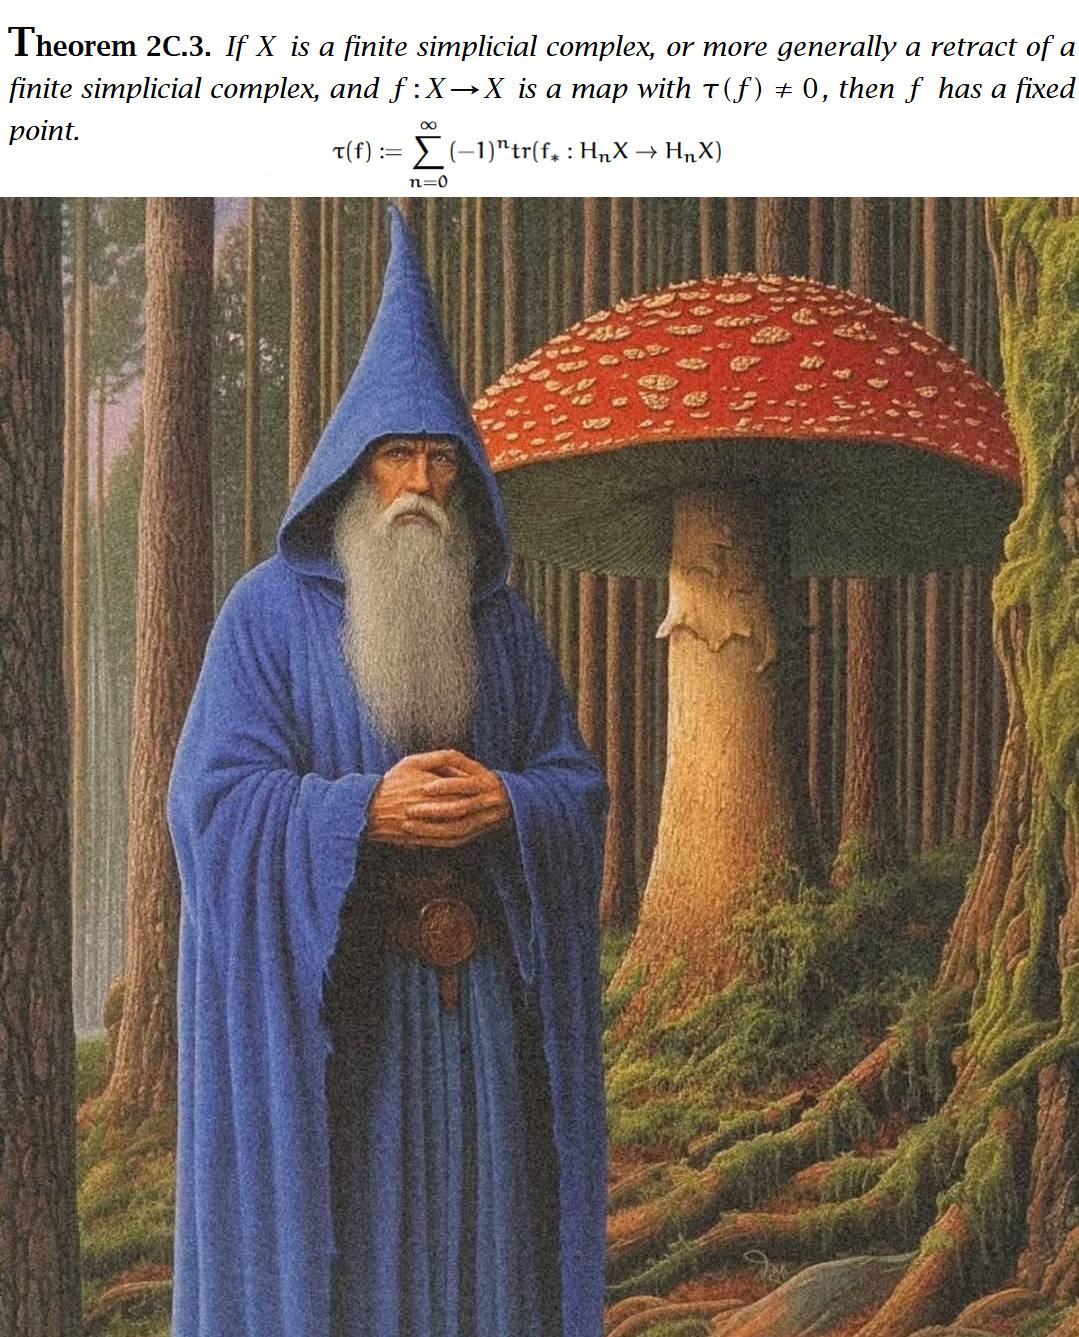
\includegraphics[width=80mm]{images/lefschetz_number.jpg}
\end{center}

\section{Cohomology}
\subsection{Cohomology Groups}
\subsection{Cup Product}

\begin{center}
    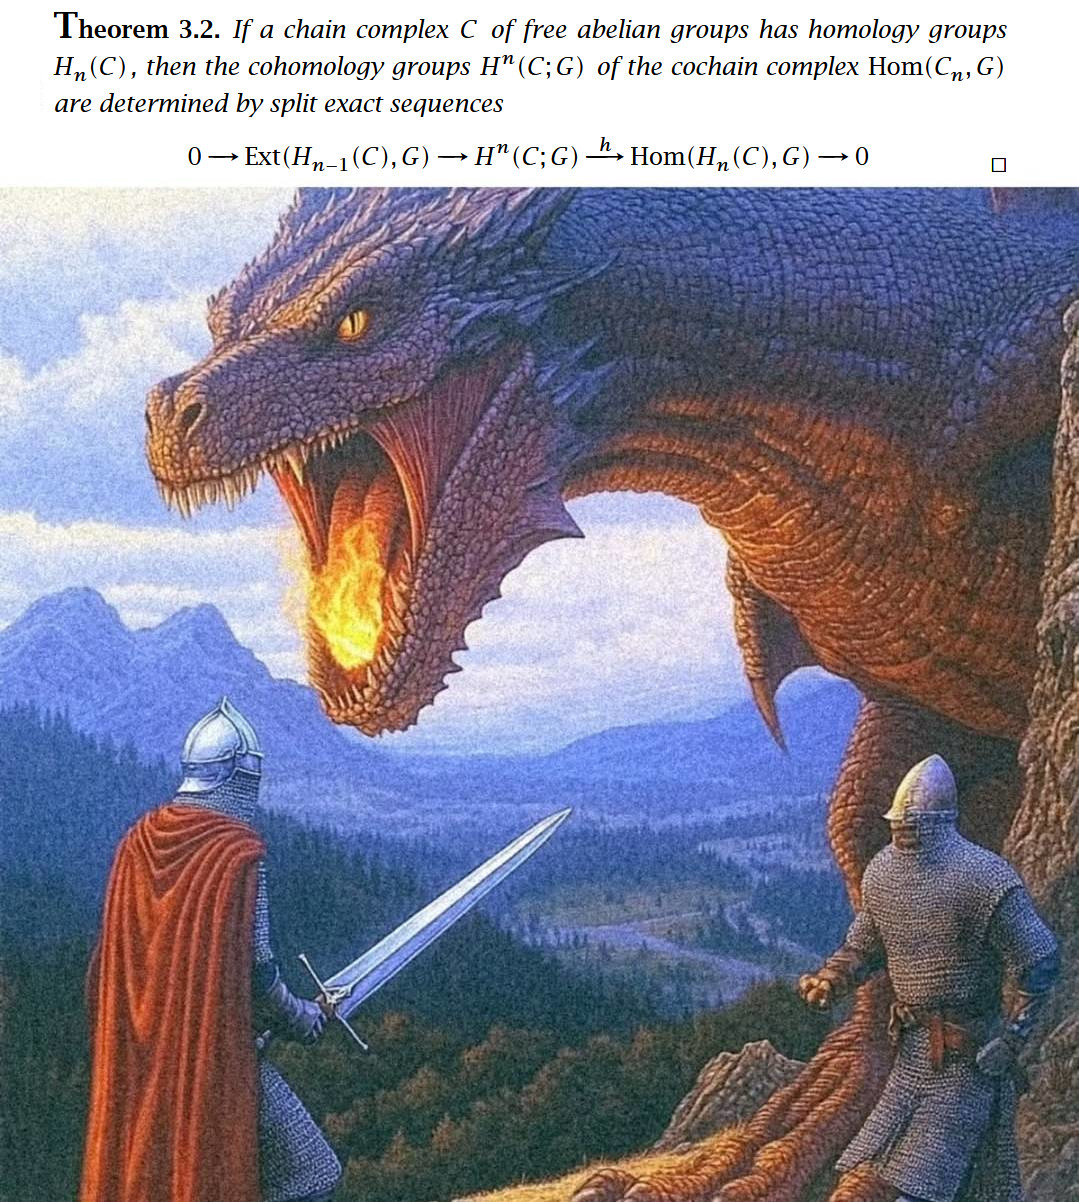
\includegraphics[width=80mm]{images/cohomology_coefficients.jpg}
\end{center}

\subsection{Poincare Duality}
\subsection{Additional Topics}
\subsubsection{Universal Coefficients for Homology}
\subsubsection{The General K\"unneth Formula}
\subsubsection{$H$-Spaces and Hopf Algebras}
\subsubsection{The Cohomology of $\SO(n)$}
\subsubsection{Bockstein Homomorphisms}
\subsubsection{Limits and $\Ext$}
\subsubsection{Transfer Homomorphisms}
\subsubsection{Local Coefficients}

\printbibliography
\nocite{*}

\clearpage
\thispagestyle{empty}

\begin{center}
    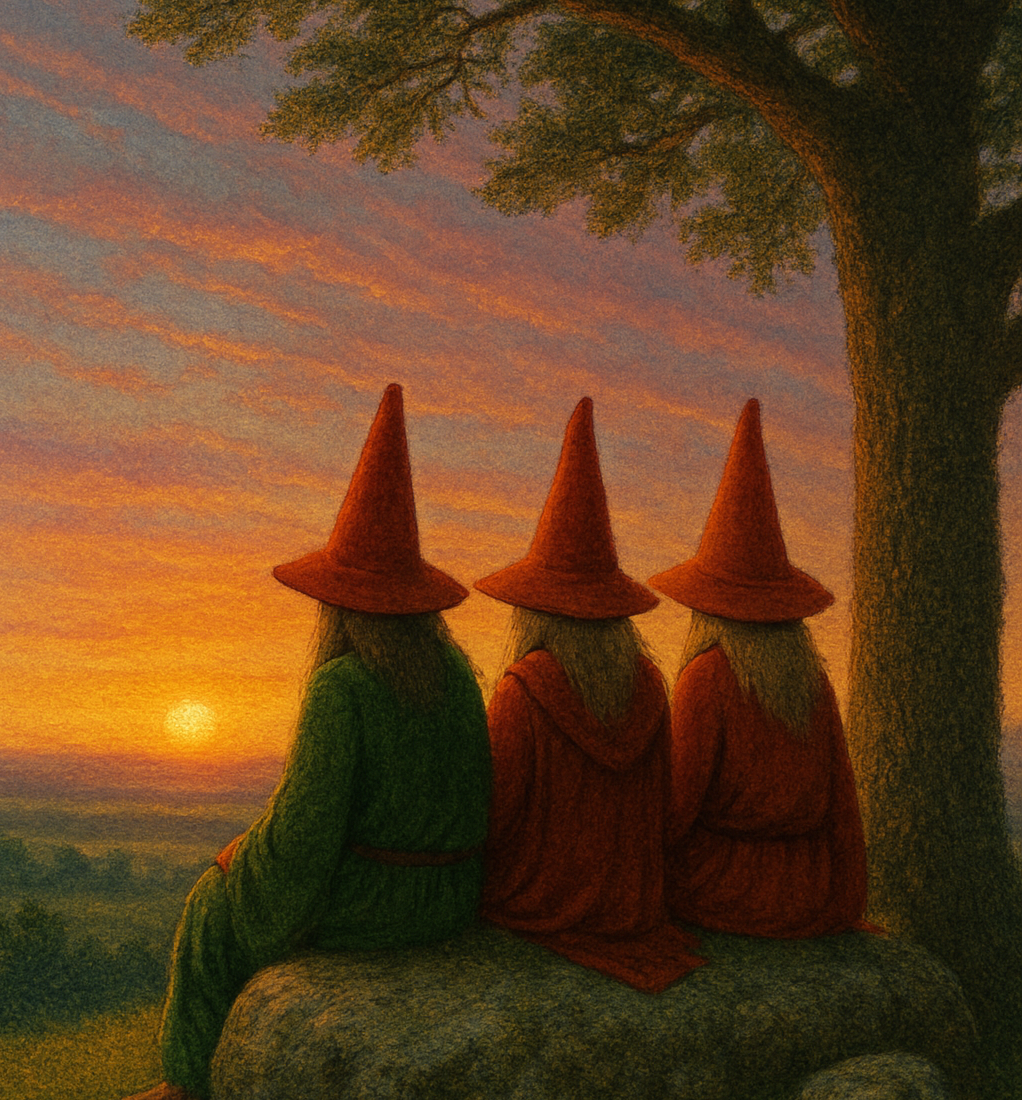
\includegraphics[width=120mm]{images/happy_ending.png}
\end{center}

\end{document}
